\documentclass[13pt, handout]{beamer}

\usetheme{Madrid}
\usecolortheme{beaver}
\setbeamertemplate{navigation symbols}{}
\setbeamertemplate{page number in head/foot}{}
\setbeamercolor*{item}{fg=red}

\usepackage[portuguese]{babel}
\usepackage{tikz}
\usepackage{ragged2e}

\title{Sistema de Gestão de Horários}
\subtitle{{}\color{black}Desenvolvimento de Sistemas de \emph{Software} 24/25}

\author[Grupo 3]{
    \begin{tabular}{lc}
        Ana Cerqueira  & \color{gray} A104188 \\
        Humberto Gomes & \color{gray} A104348 \\
        João Torres     & \color{gray} A95748 \\
        José Lopes     & \color{gray} A104541 \\
        José Matos     & \color{gray} A100612
    \end{tabular}
}

\institute[DIUM]{
    Departamento de Informática -- Escola de Engenharia -- Univerisidade do Minho \\
    Licenciatura em Engenharia Informática
}

\date[2025/01/07]{\scriptsize 7 de janeiro de 2025}

\begin{document}
\frame{\titlepage}

\begin{frame}{Índice}
    \tableofcontents
\end{frame}

\justifying

\section{Análise de Requisitos}

\begin{frame}{Análise de Requisitos -- O Problema}
    É pretendido o desenvolvimento de \emph{software} onde:

    \vspace{0.5cm}
    \begin{itemize}
        \item Diretores de curso sejam capazes de definir os horários dos alunos;
        \item Os alunos sejam capazes de consultar os seus horários.
    \end{itemize}
\end{frame}

\begin{frame}{Análise de Requisitos -- Modelo de Domínio}
    \centering
    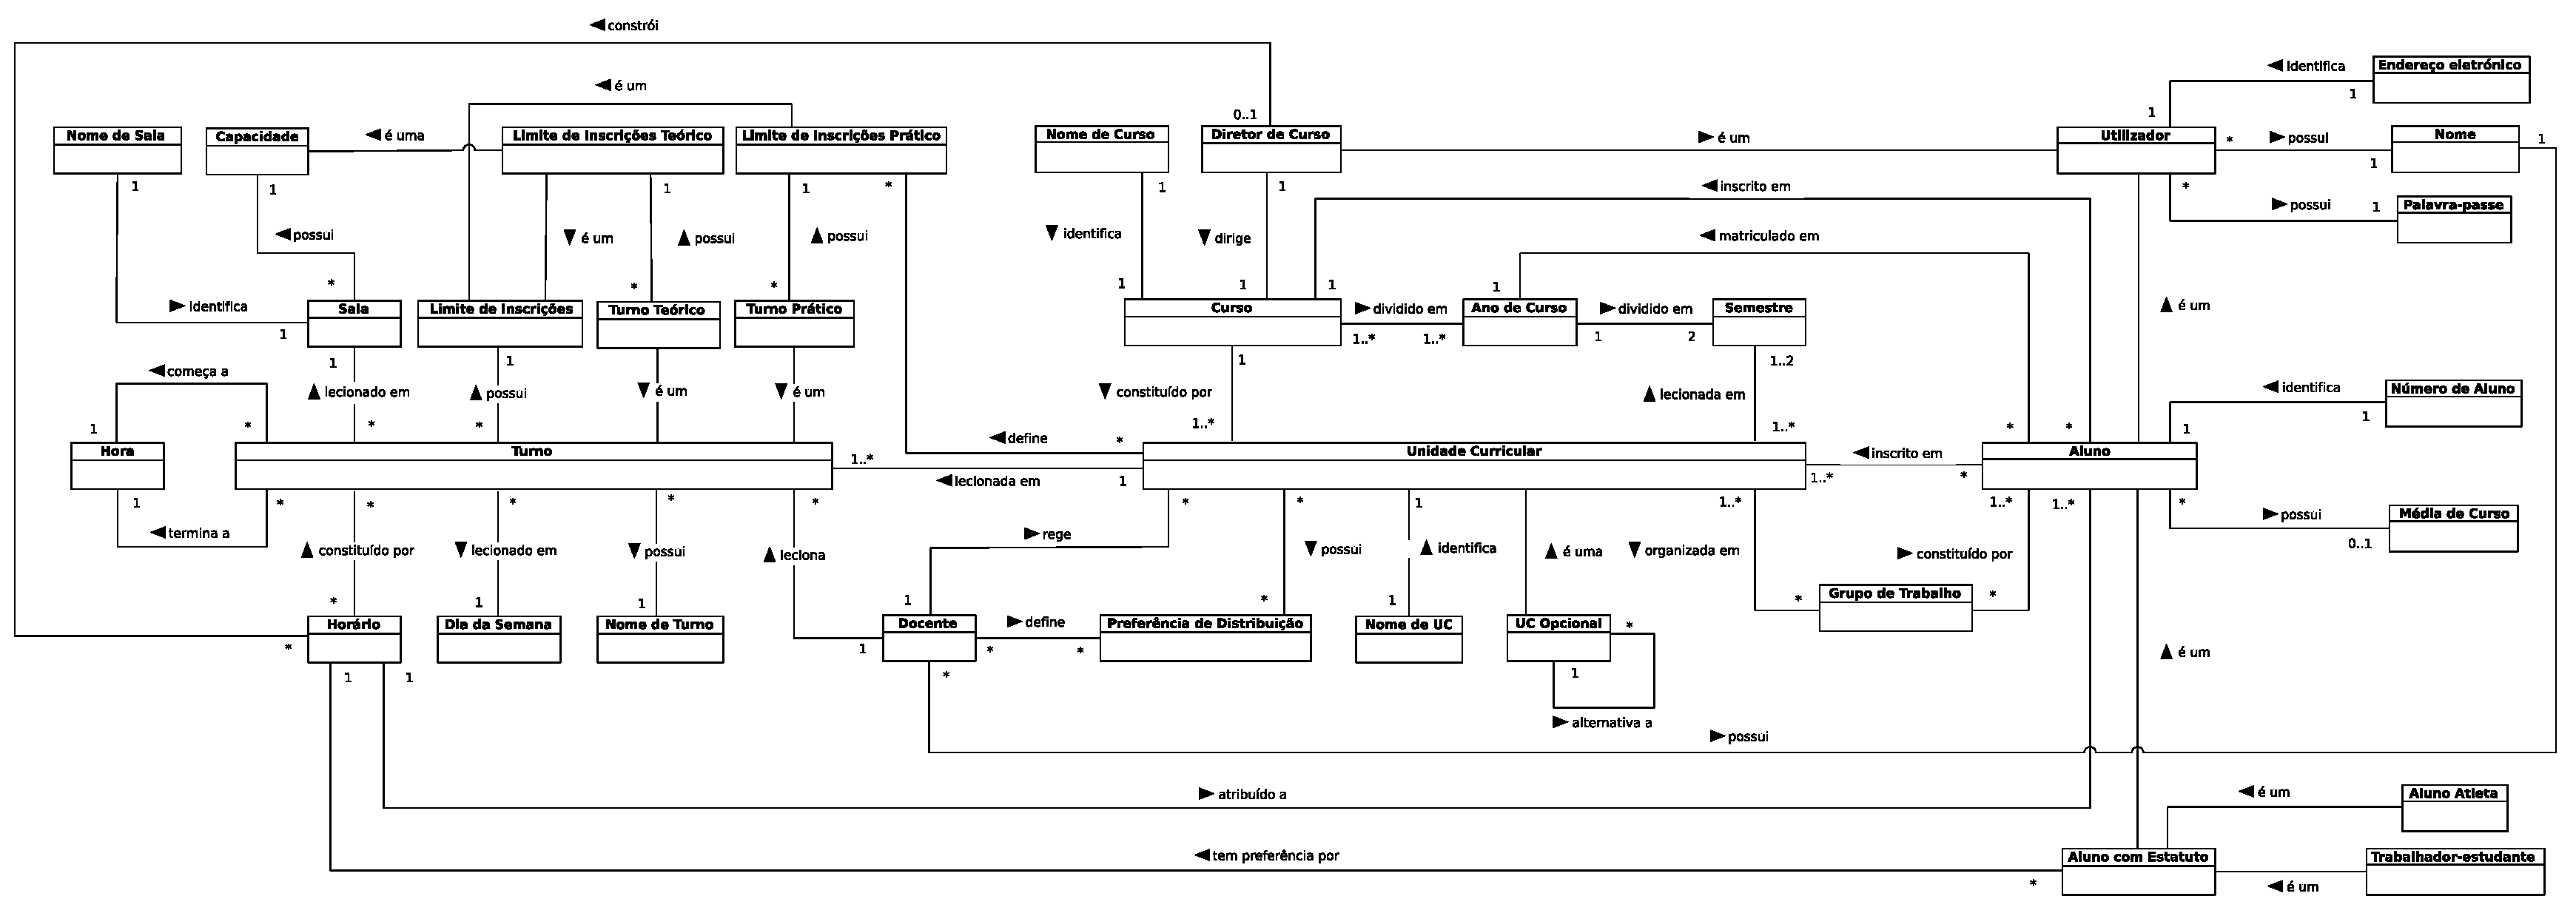
\includegraphics[scale=0.20]{Imagens/Modelos/ModeloDominio.svg.eps} \\
    {\scriptsize Modelo de Domínio construído.}

    \vspace{0.5cm}
    \begin{itemize}
        \item Construído com conhecimento próprio;
        \item Informação do enunciado para esclarecer detalhes;
        \item Definição de restrições sobre as relações.
    \end{itemize}
\end{frame}

\begin{frame}{Análise de Requisitos -- Identificação dos Casos de Uso}
    \centering

    \begin{minipage}{0.45\textwidth}
        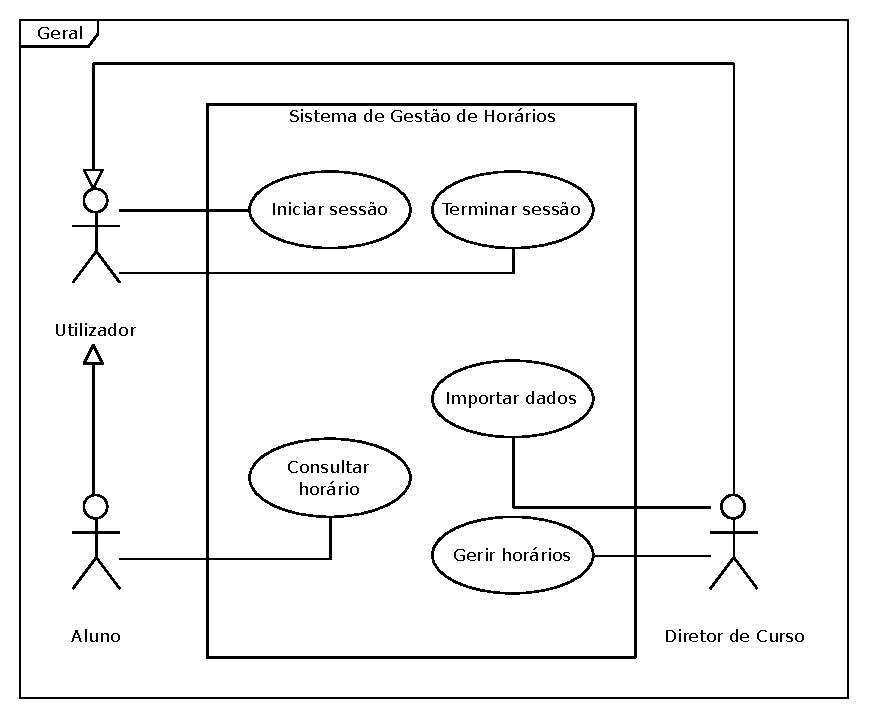
\includegraphics[width=\textwidth]{Imagens/Modelos/UseCasesGeral.eps}
    \end{minipage}
    \hspace{0.5cm}
    \begin{minipage}{0.45\textwidth}
        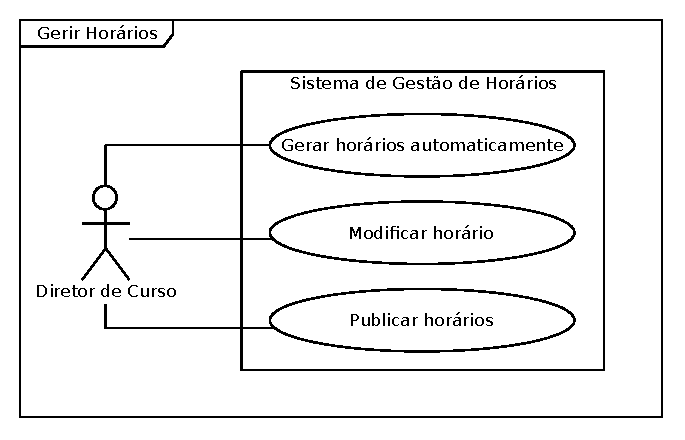
\includegraphics[width=\textwidth]{Imagens/Modelos/UseCasesGerirHorarios.eps}
    \end{minipage} \\
    \vspace{0.25cm}
    {\scriptsize Dois dos diagramas de casos de uso construídos.}

    \vspace{0.5cm}
    \begin{itemize}
        \item Identificação dos atores e das operações suportadas;
        \item Construção de diagramas.
    \end{itemize}
\end{frame}

\begin{frame}{Análise de Requisitos -- Especificação dos Casos de Uso}
    \centering
    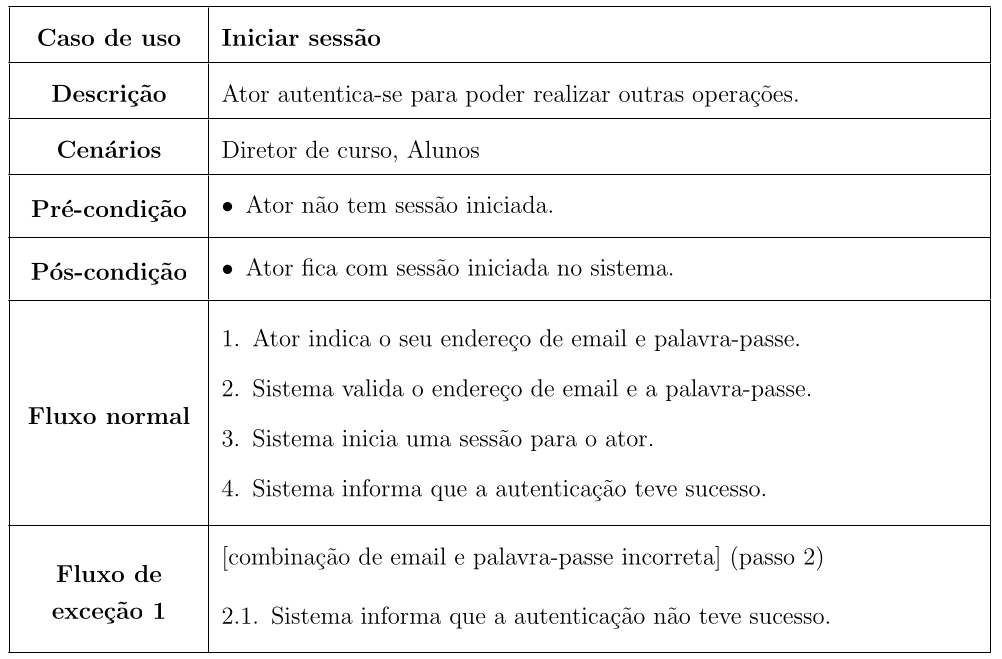
\includegraphics[width=0.9\textwidth]{Imagens/Slides/UseCase.png} \\
    {\scriptsize Exemplo de um caso de uso especificado.}
\end{frame}

\section{Modelação conceptual}

\begin{frame}{\large Modelação conceptual -- Definição da API da Camada de Negócio}
    \centering
    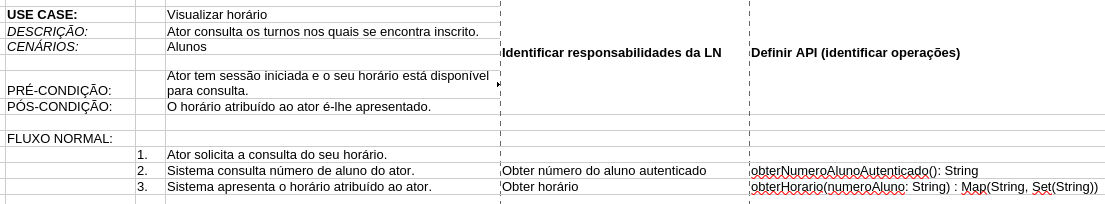
\includegraphics[width=\textwidth]{Imagens/Slides/API.png} \\
    {\scriptsize Definição da API da camada de negócio para o caso de uso "Visualizar Horário"{}.}

    \vspace{0.5cm}
    \begin{itemize}
        \item Identificação das responsabilidades da camada de negócio;
        \item Definição da sua API.
    \end{itemize}
\end{frame}

\begin{frame}{\large Modelação conceptual -- Divisão das Operações por Subsistemas}
    \centering
    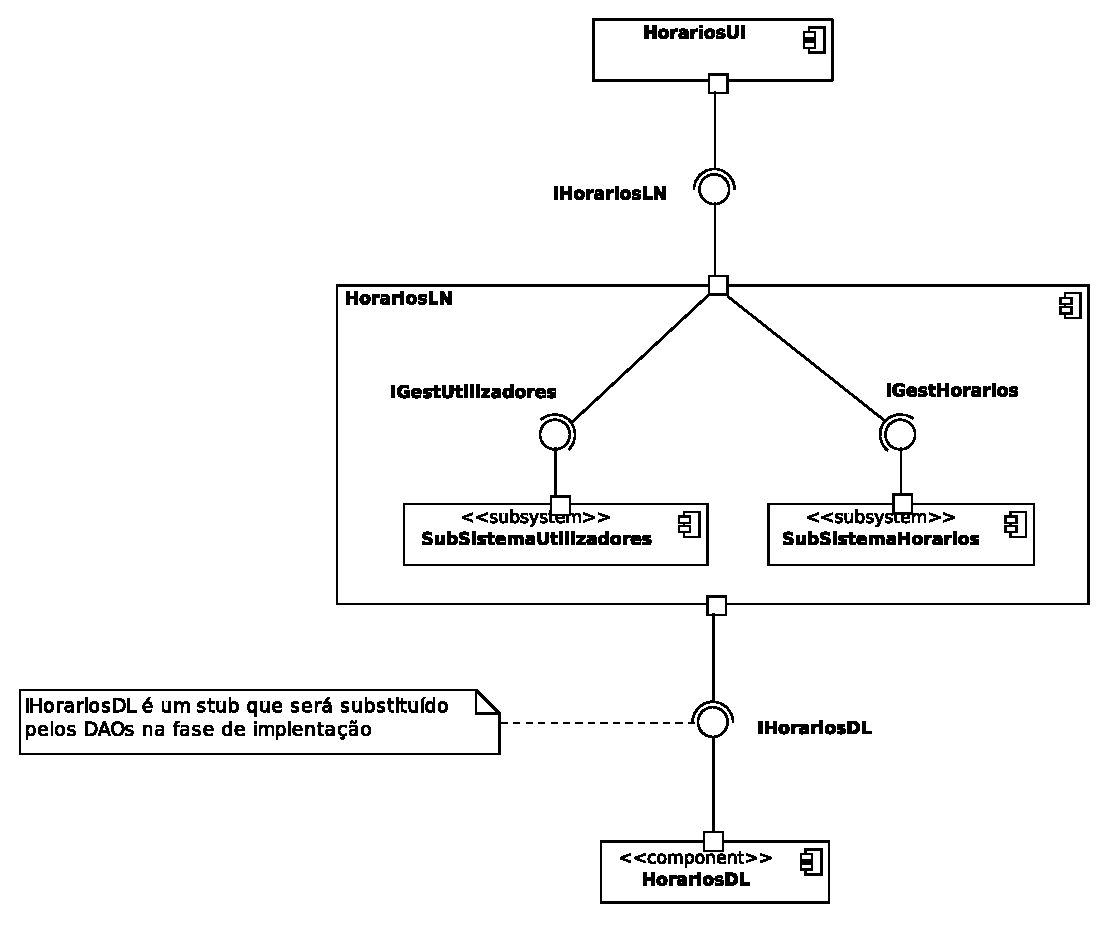
\includegraphics[width=0.7\textwidth]{Imagens/Modelos/Componentes.svg.eps} \\
    {\scriptsize Primeiro diagrama de componentes construído.}
\end{frame}

\begin{frame}{Modelação conceptual -- Diagramas de Classe}
    \centering
    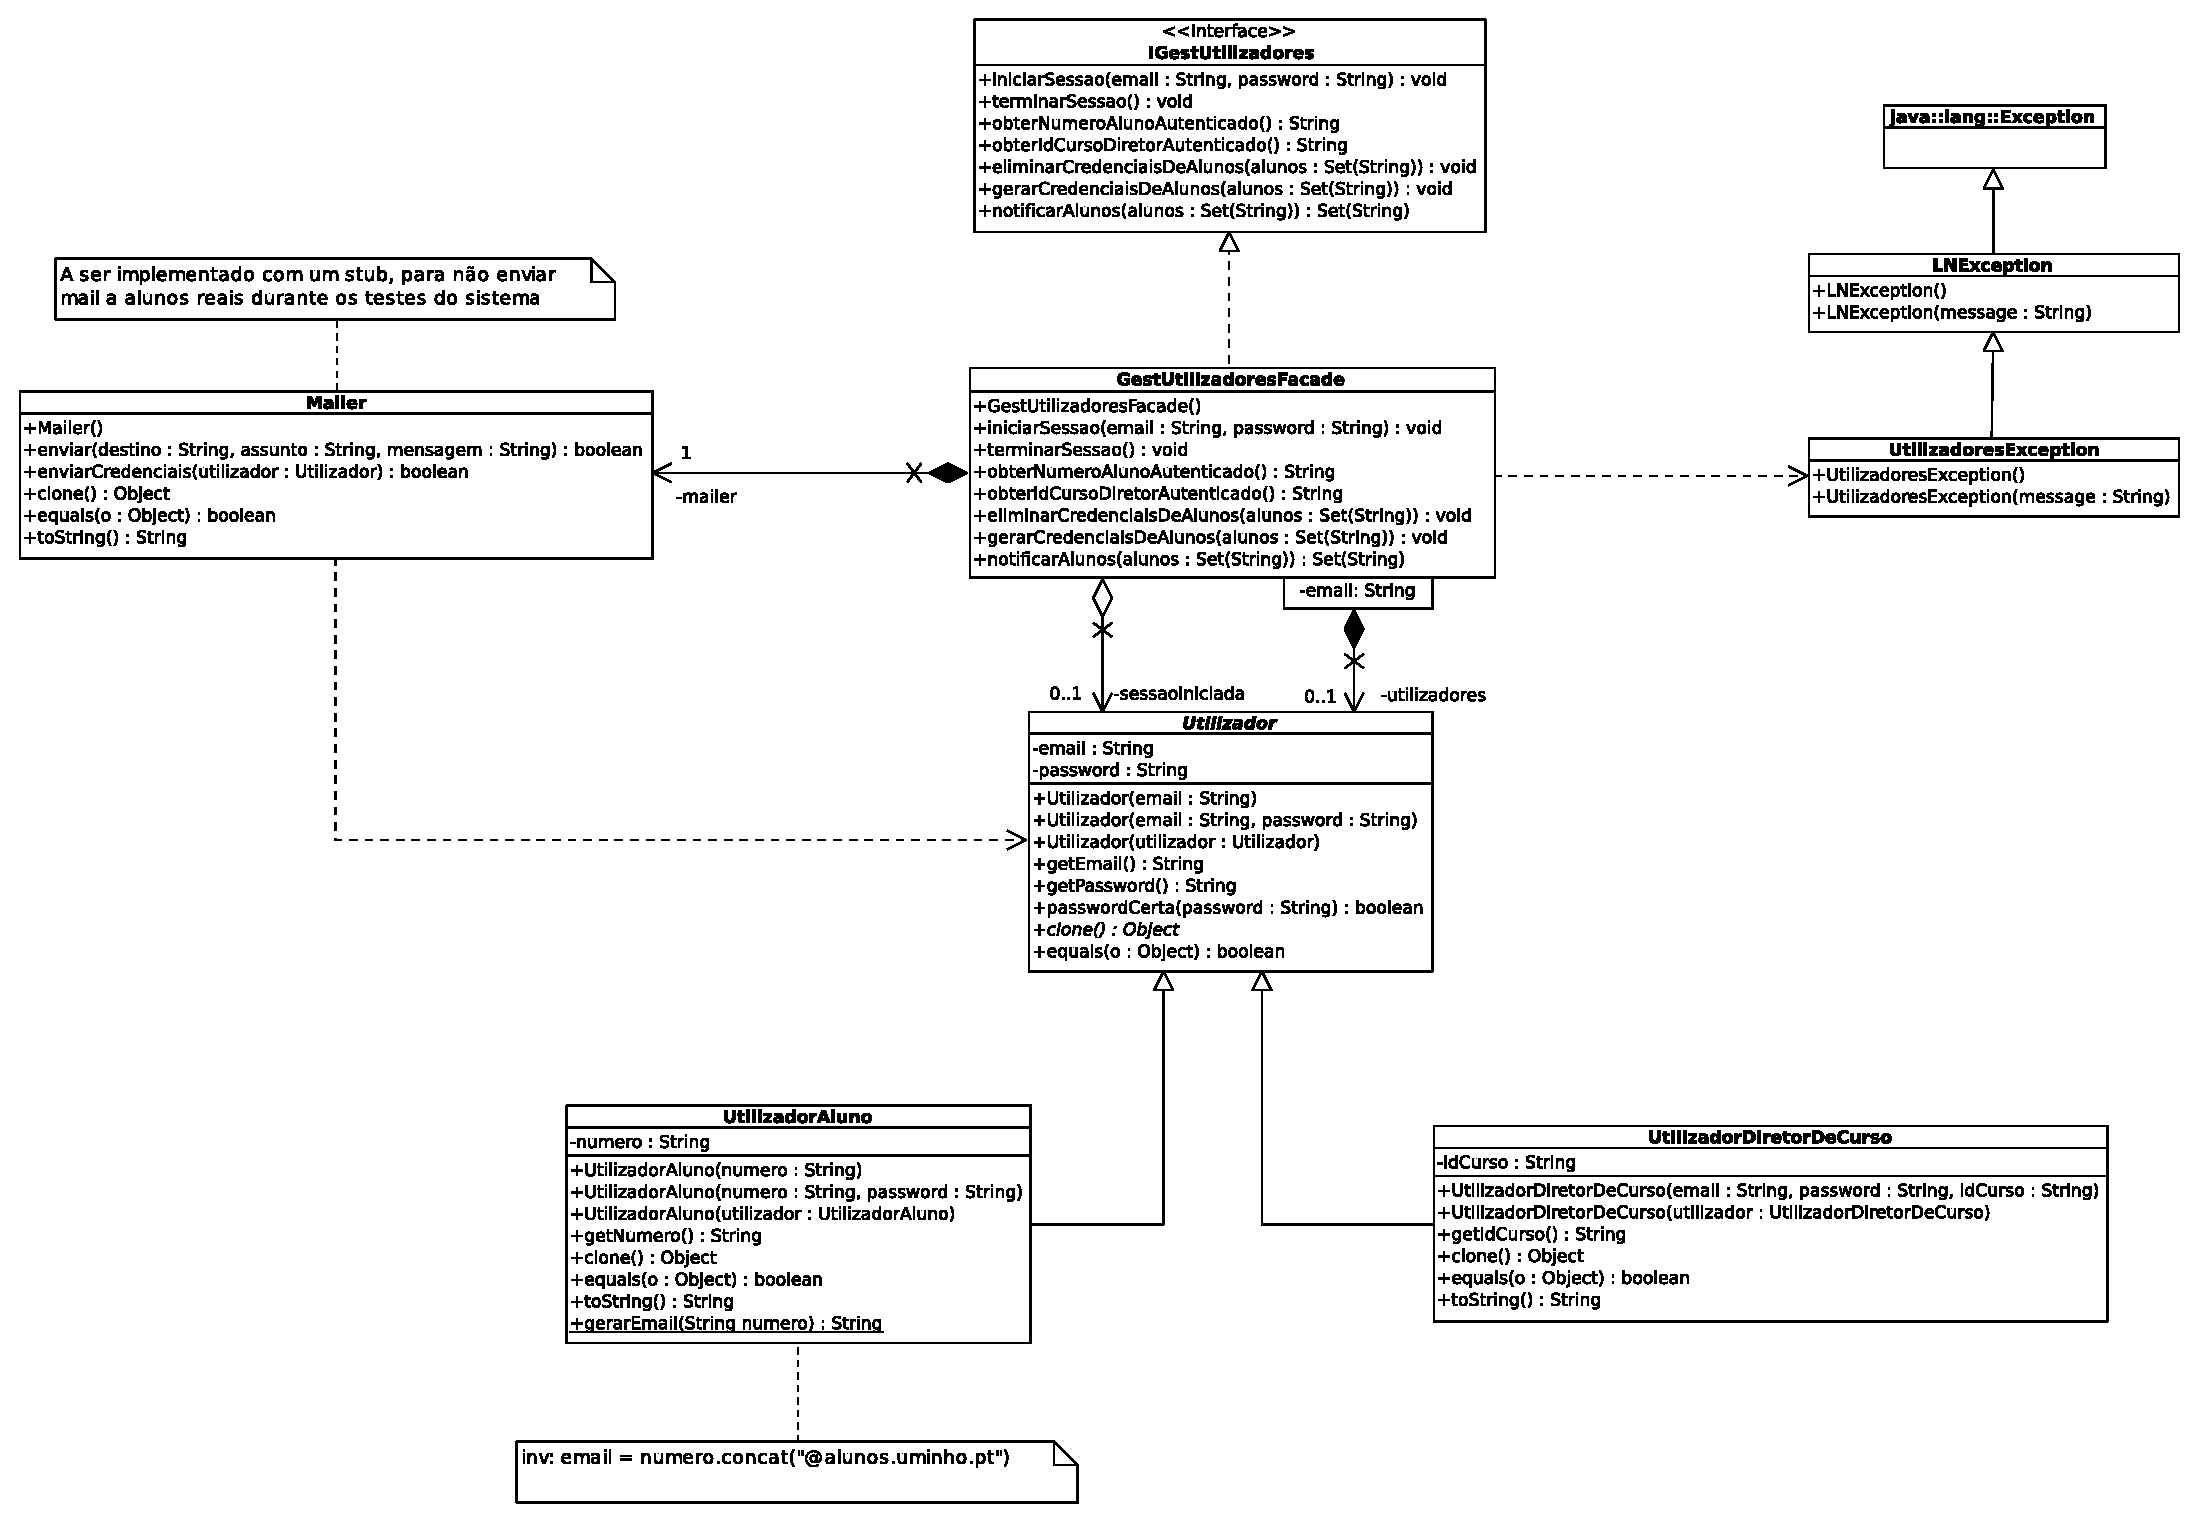
\includegraphics[width=0.8\textwidth]{Imagens/Modelos/Utilizadores.svg.eps} \\
    {\scriptsize Diagrama de classes do subsistema dos utilizadores.}
\end{frame}

\begin{frame}{Modelação conceptual -- Diagramas de Sequência}
    \centering
    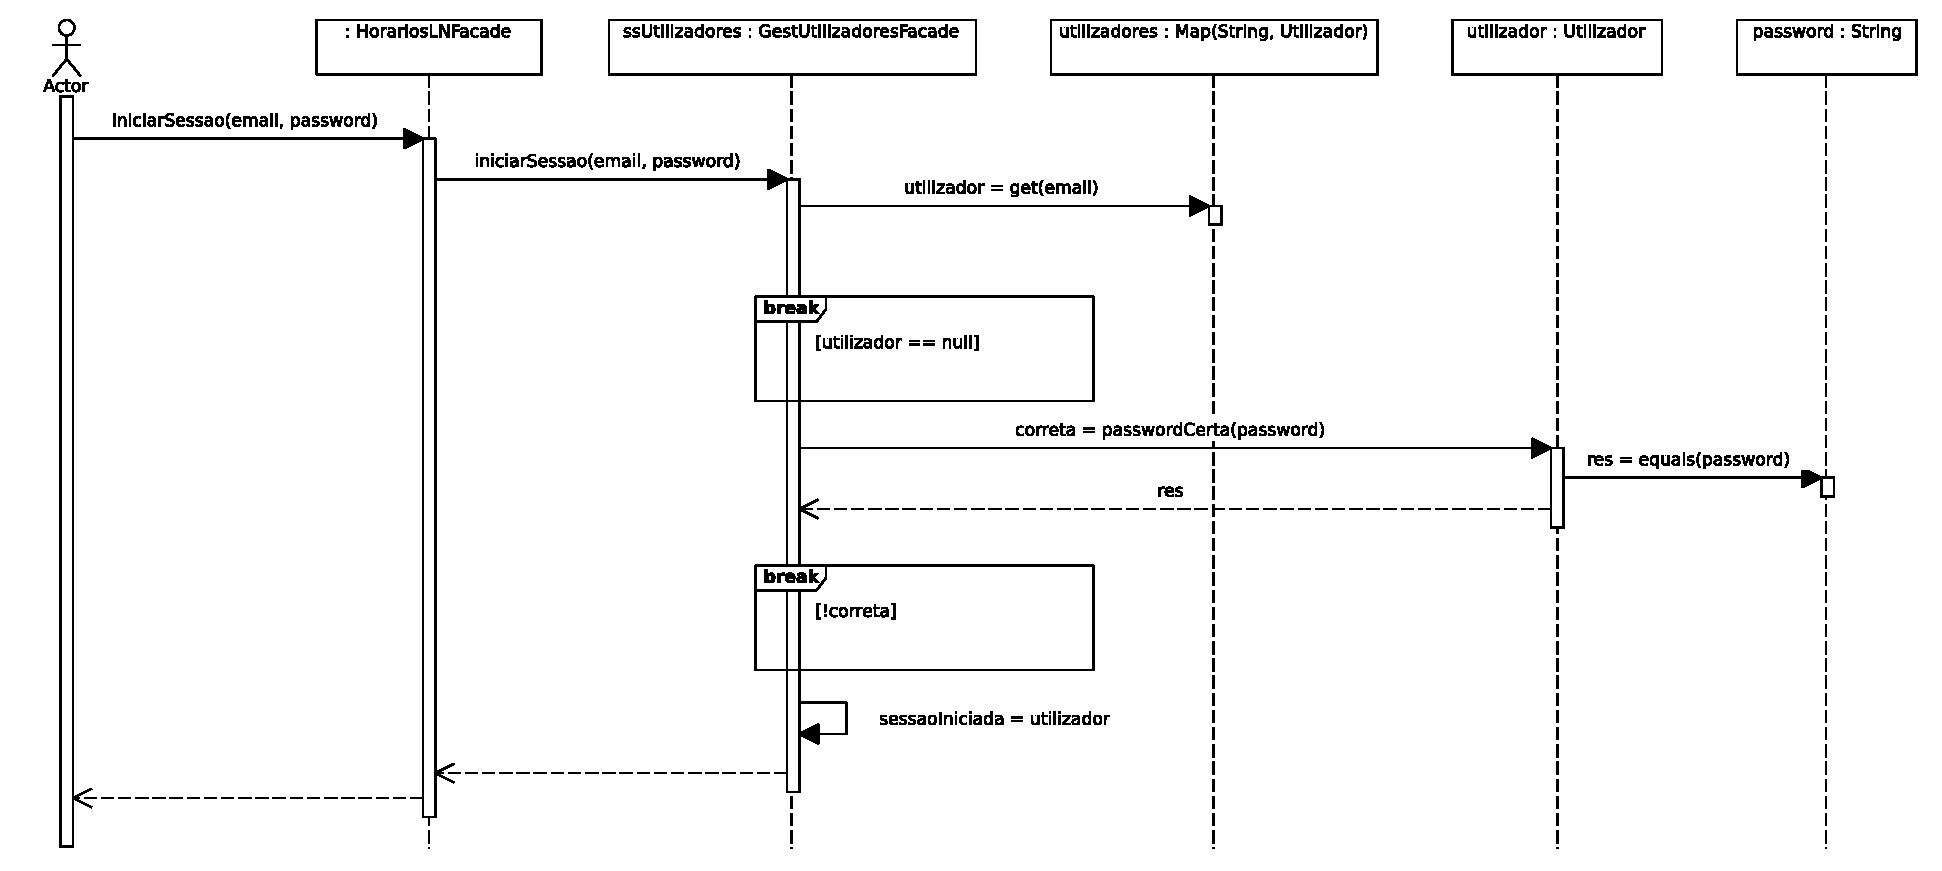
\includegraphics[scale=0.35]{Imagens/Modelos/iniciarSessao.svg.eps} \\
    {\scriptsize Diagrama de sequência da operação \texttt{iniciarSessao}.}

    \vspace{0.5cm}
    \begin{itemize}
        \item Modelação comportamental de todas as operações da camada de negócio.
    \end{itemize}
\end{frame}

\begin{frame}{Modelação conceptual -- Geração Automática de Horários}
    \centering
    
    \begin{itemize}
        \item Geração de um problema de programação inteira;
        \item Resolução um \emph{solver} externo (\emph{GNU Linear Programming Kit});
        \item Protótipo descartável desenvolvido em Python.
    \end{itemize}
\end{frame}

\section{Implementação}

\begin{frame}{Implementação -- Adição de uma BD Relacional}
    \centering
    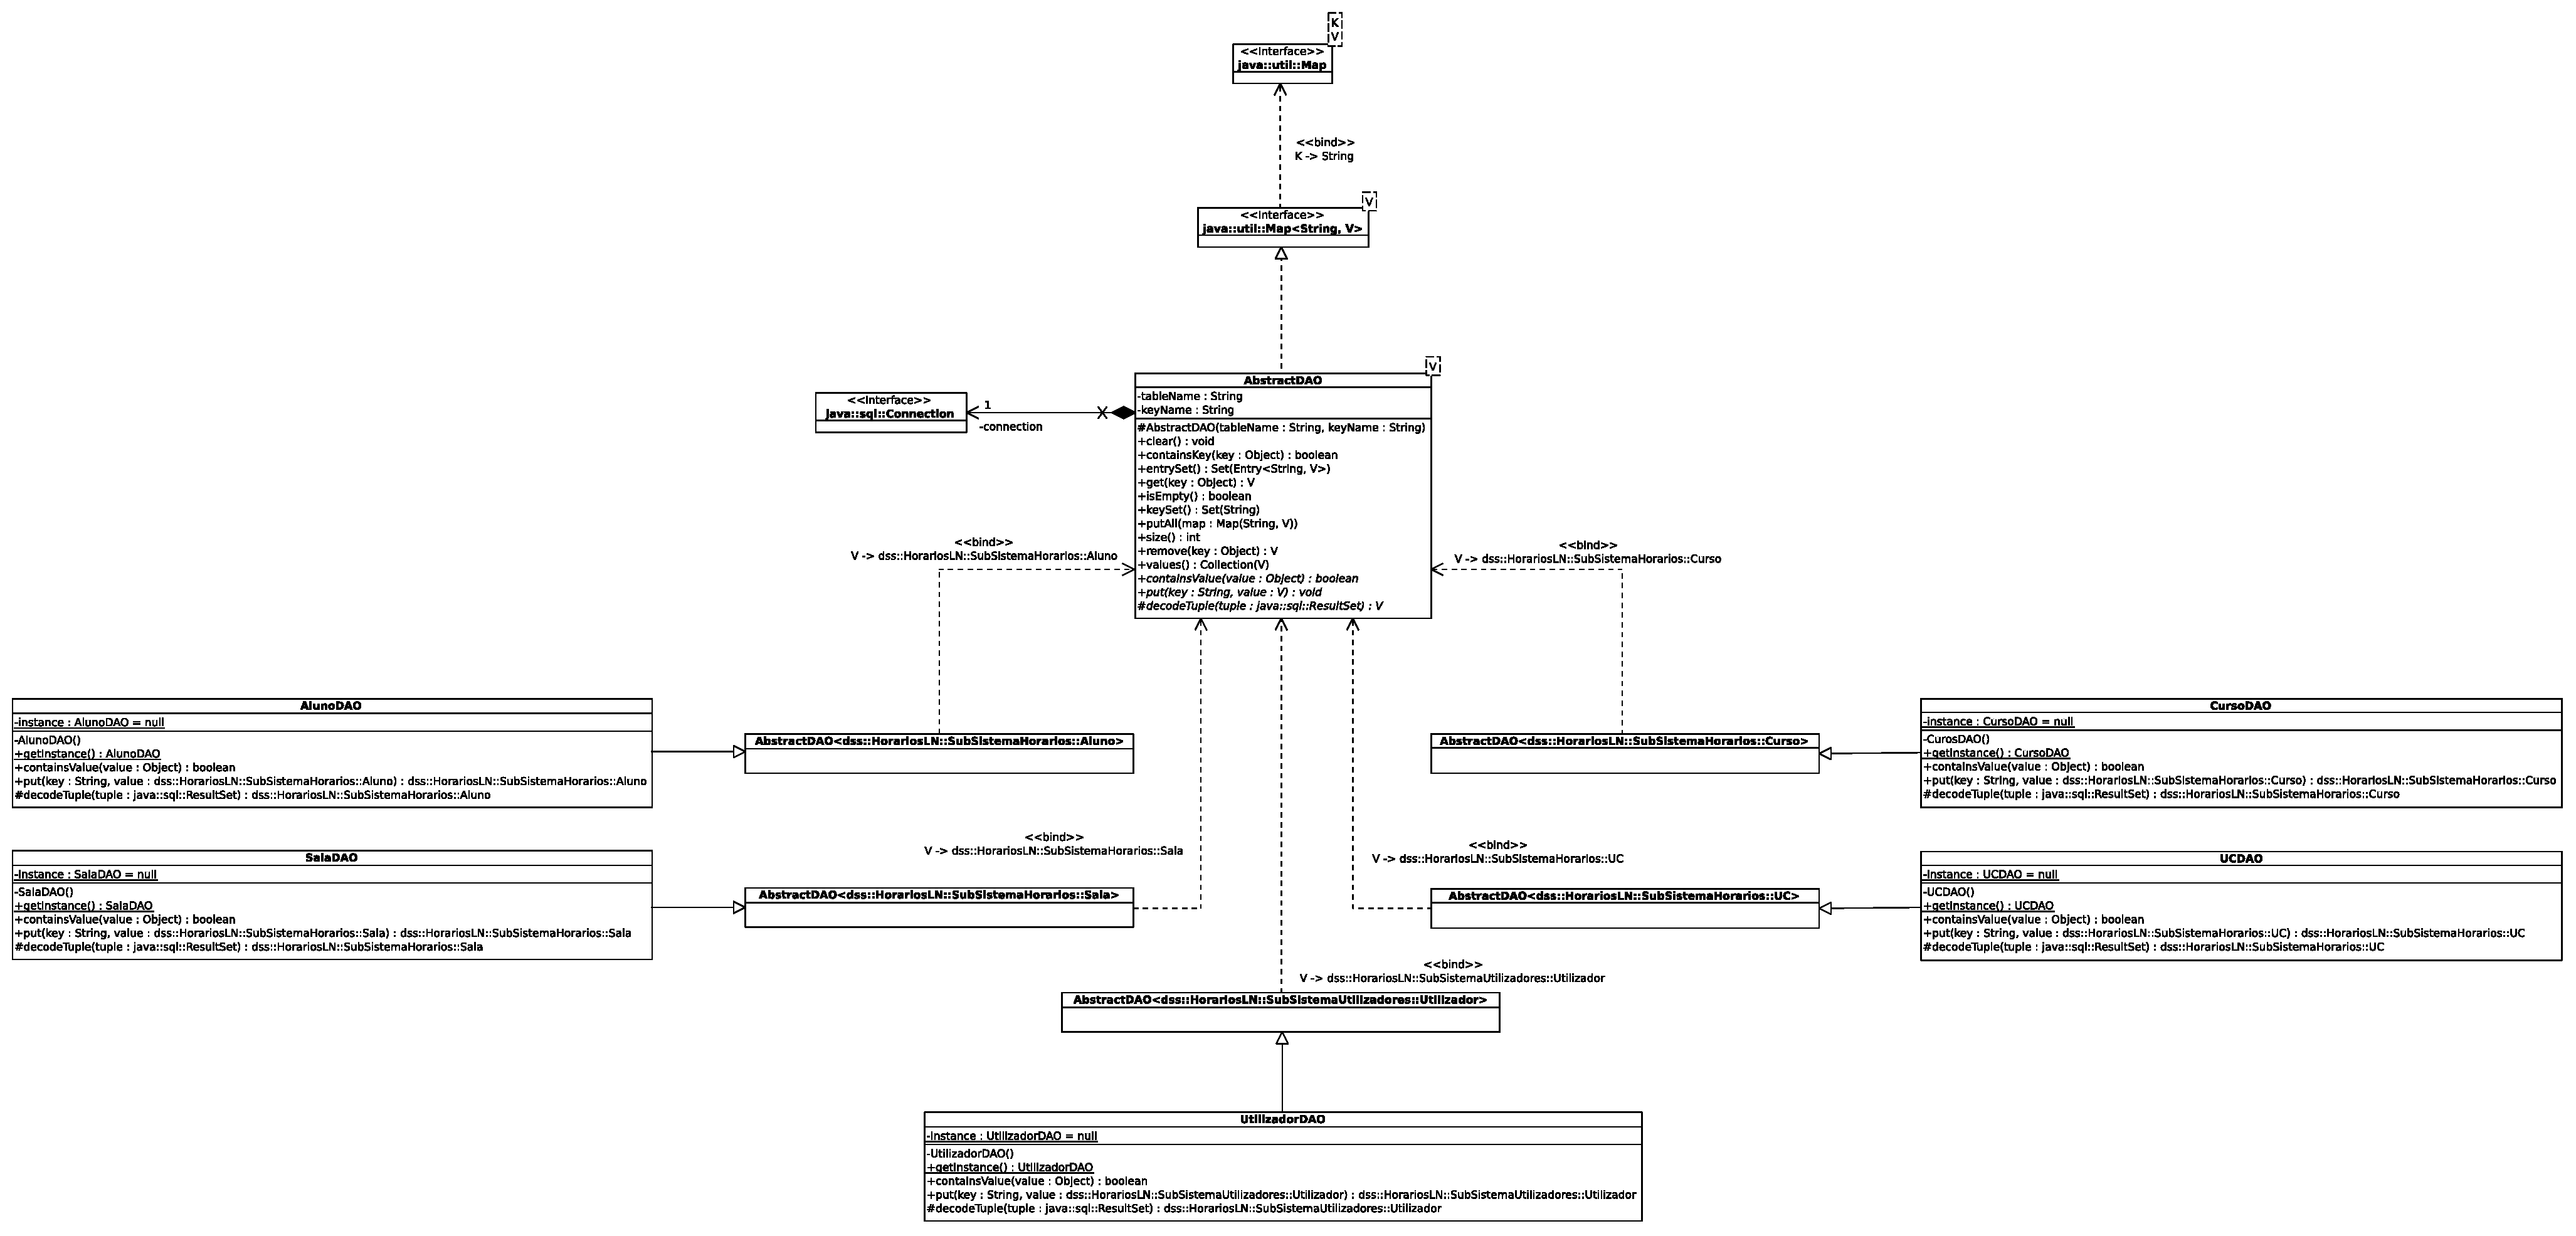
\includegraphics[scale=0.175]{Imagens/Modelos/HierarquiaDAO.svg.eps}
    {\scriptsize Hierarquia do DAOs, utilizados para \emph{Object-Relational Mapping}.}
\end{frame}

\begin{frame}{Implementação -- Arquitetura final}
    \centering

    \begin{minipage}{0.45\textwidth}
        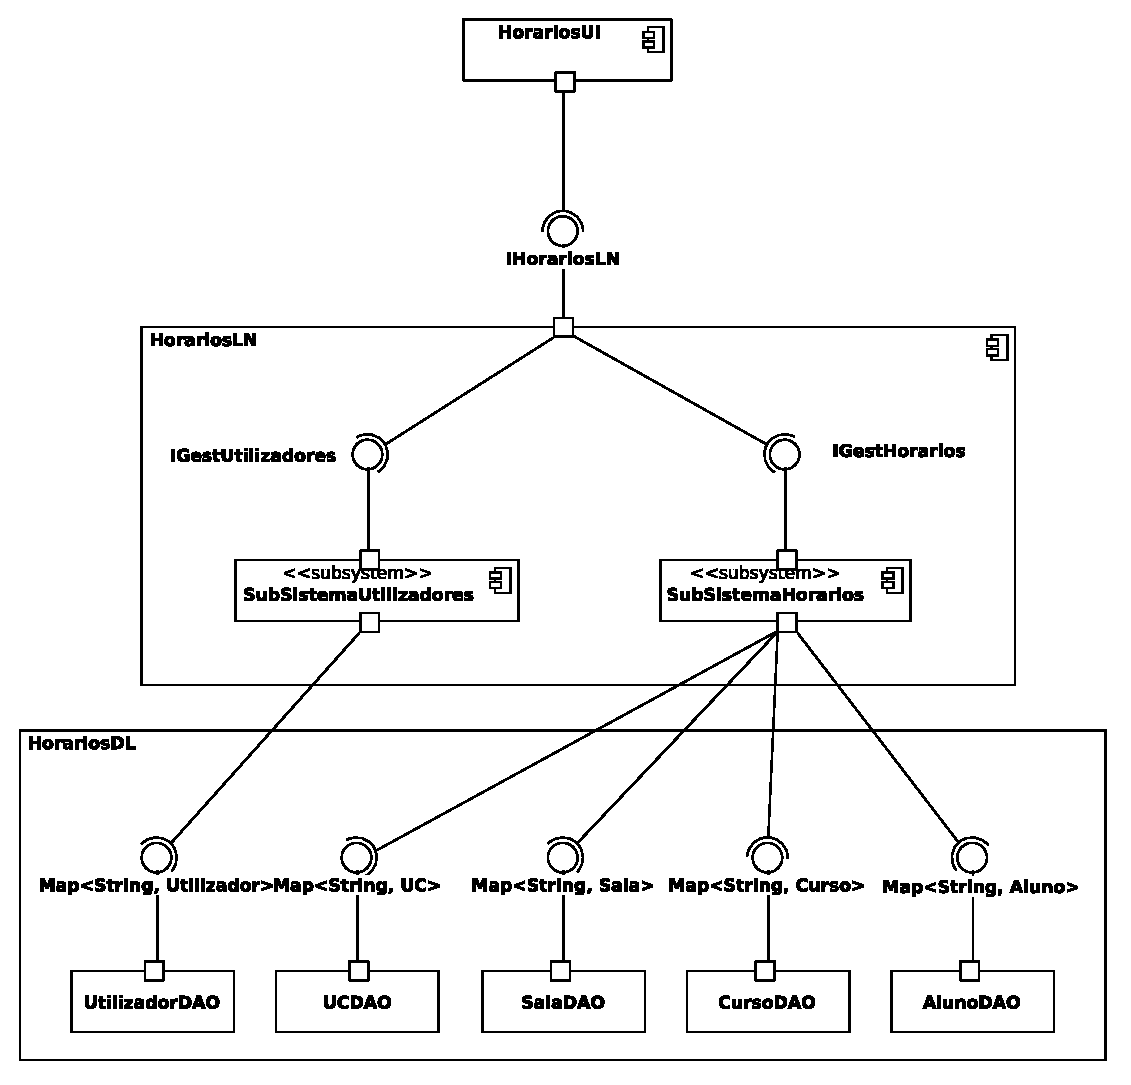
\includegraphics[width=\textwidth]{Imagens/Modelos/ComponentesDAO.svg.eps}
    \end{minipage}
    \hspace{0.5cm}
    \begin{minipage}{0.45\textwidth}
        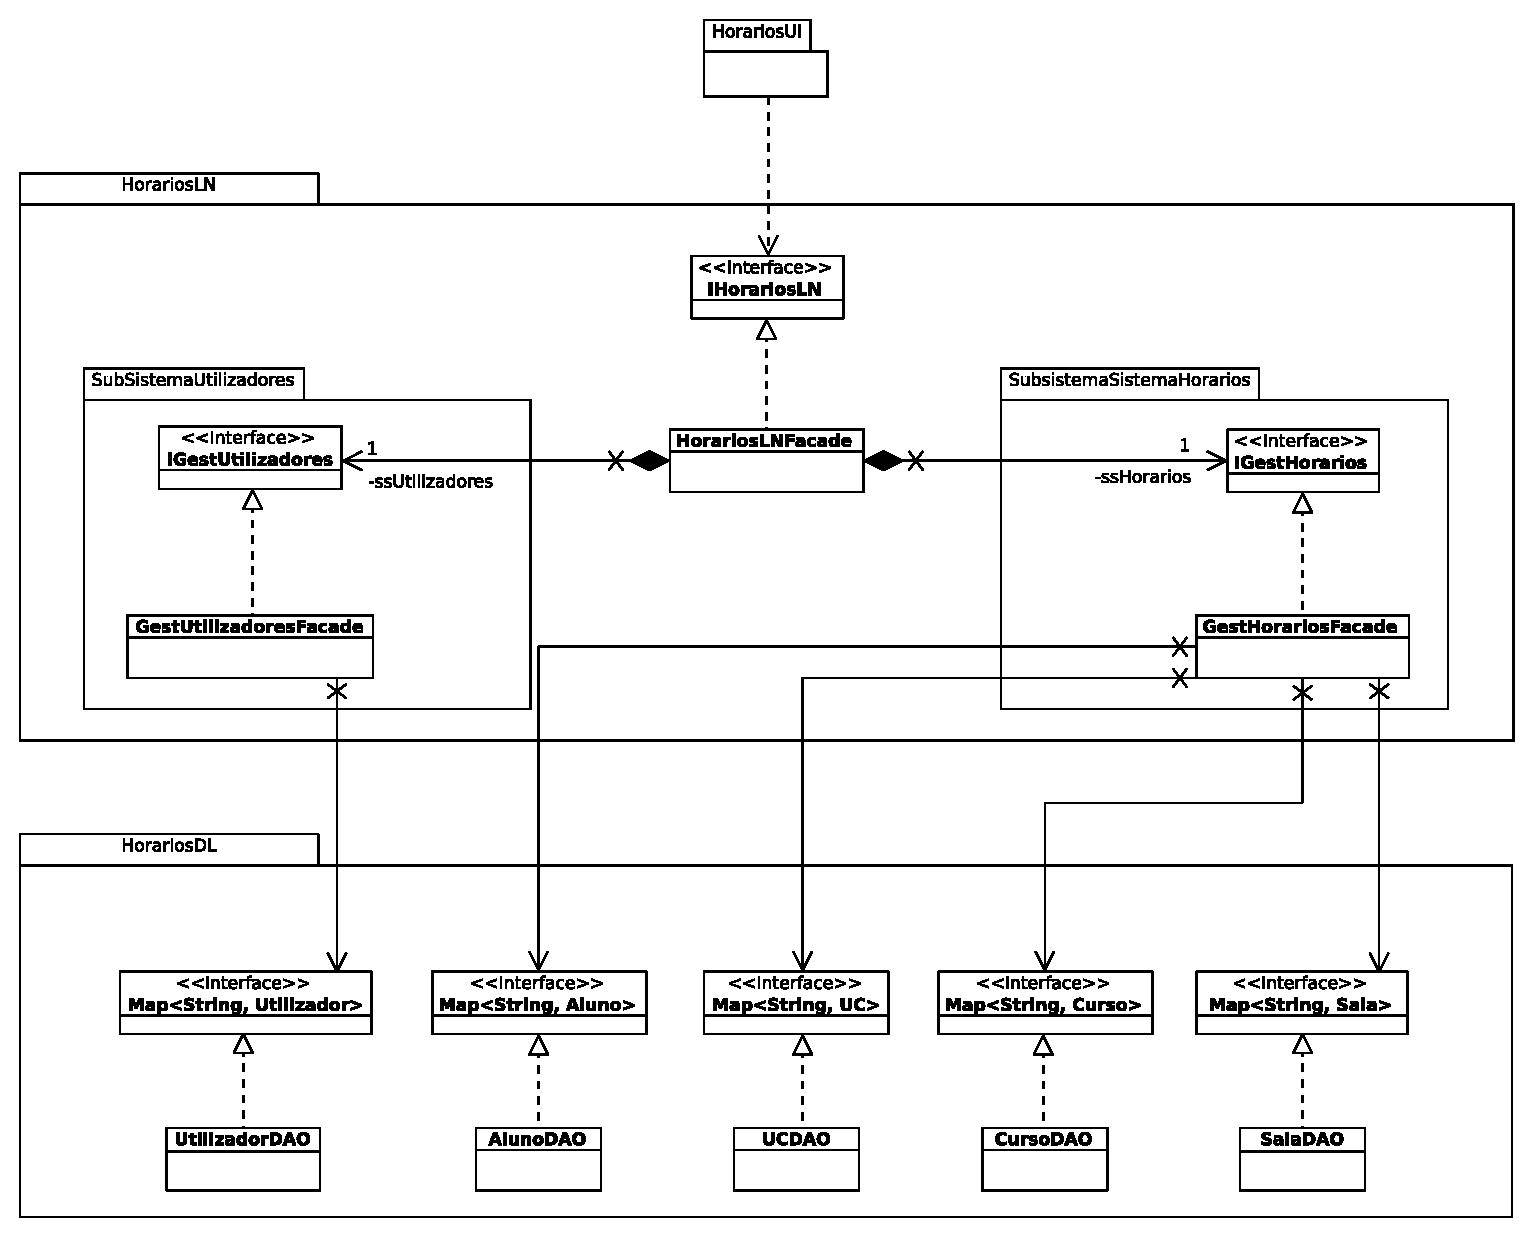
\includegraphics[width=\textwidth]{Imagens/Modelos/GeralDAO.svg.eps}
    \end{minipage} \\
    \vspace{0.25cm}
    {\scriptsize Diagramas de componentes de \emph{packages} finais.}
\end{frame}

\begin{frame}{Implementação -- Alterações aos Diagramas de Classe}
    \centering
    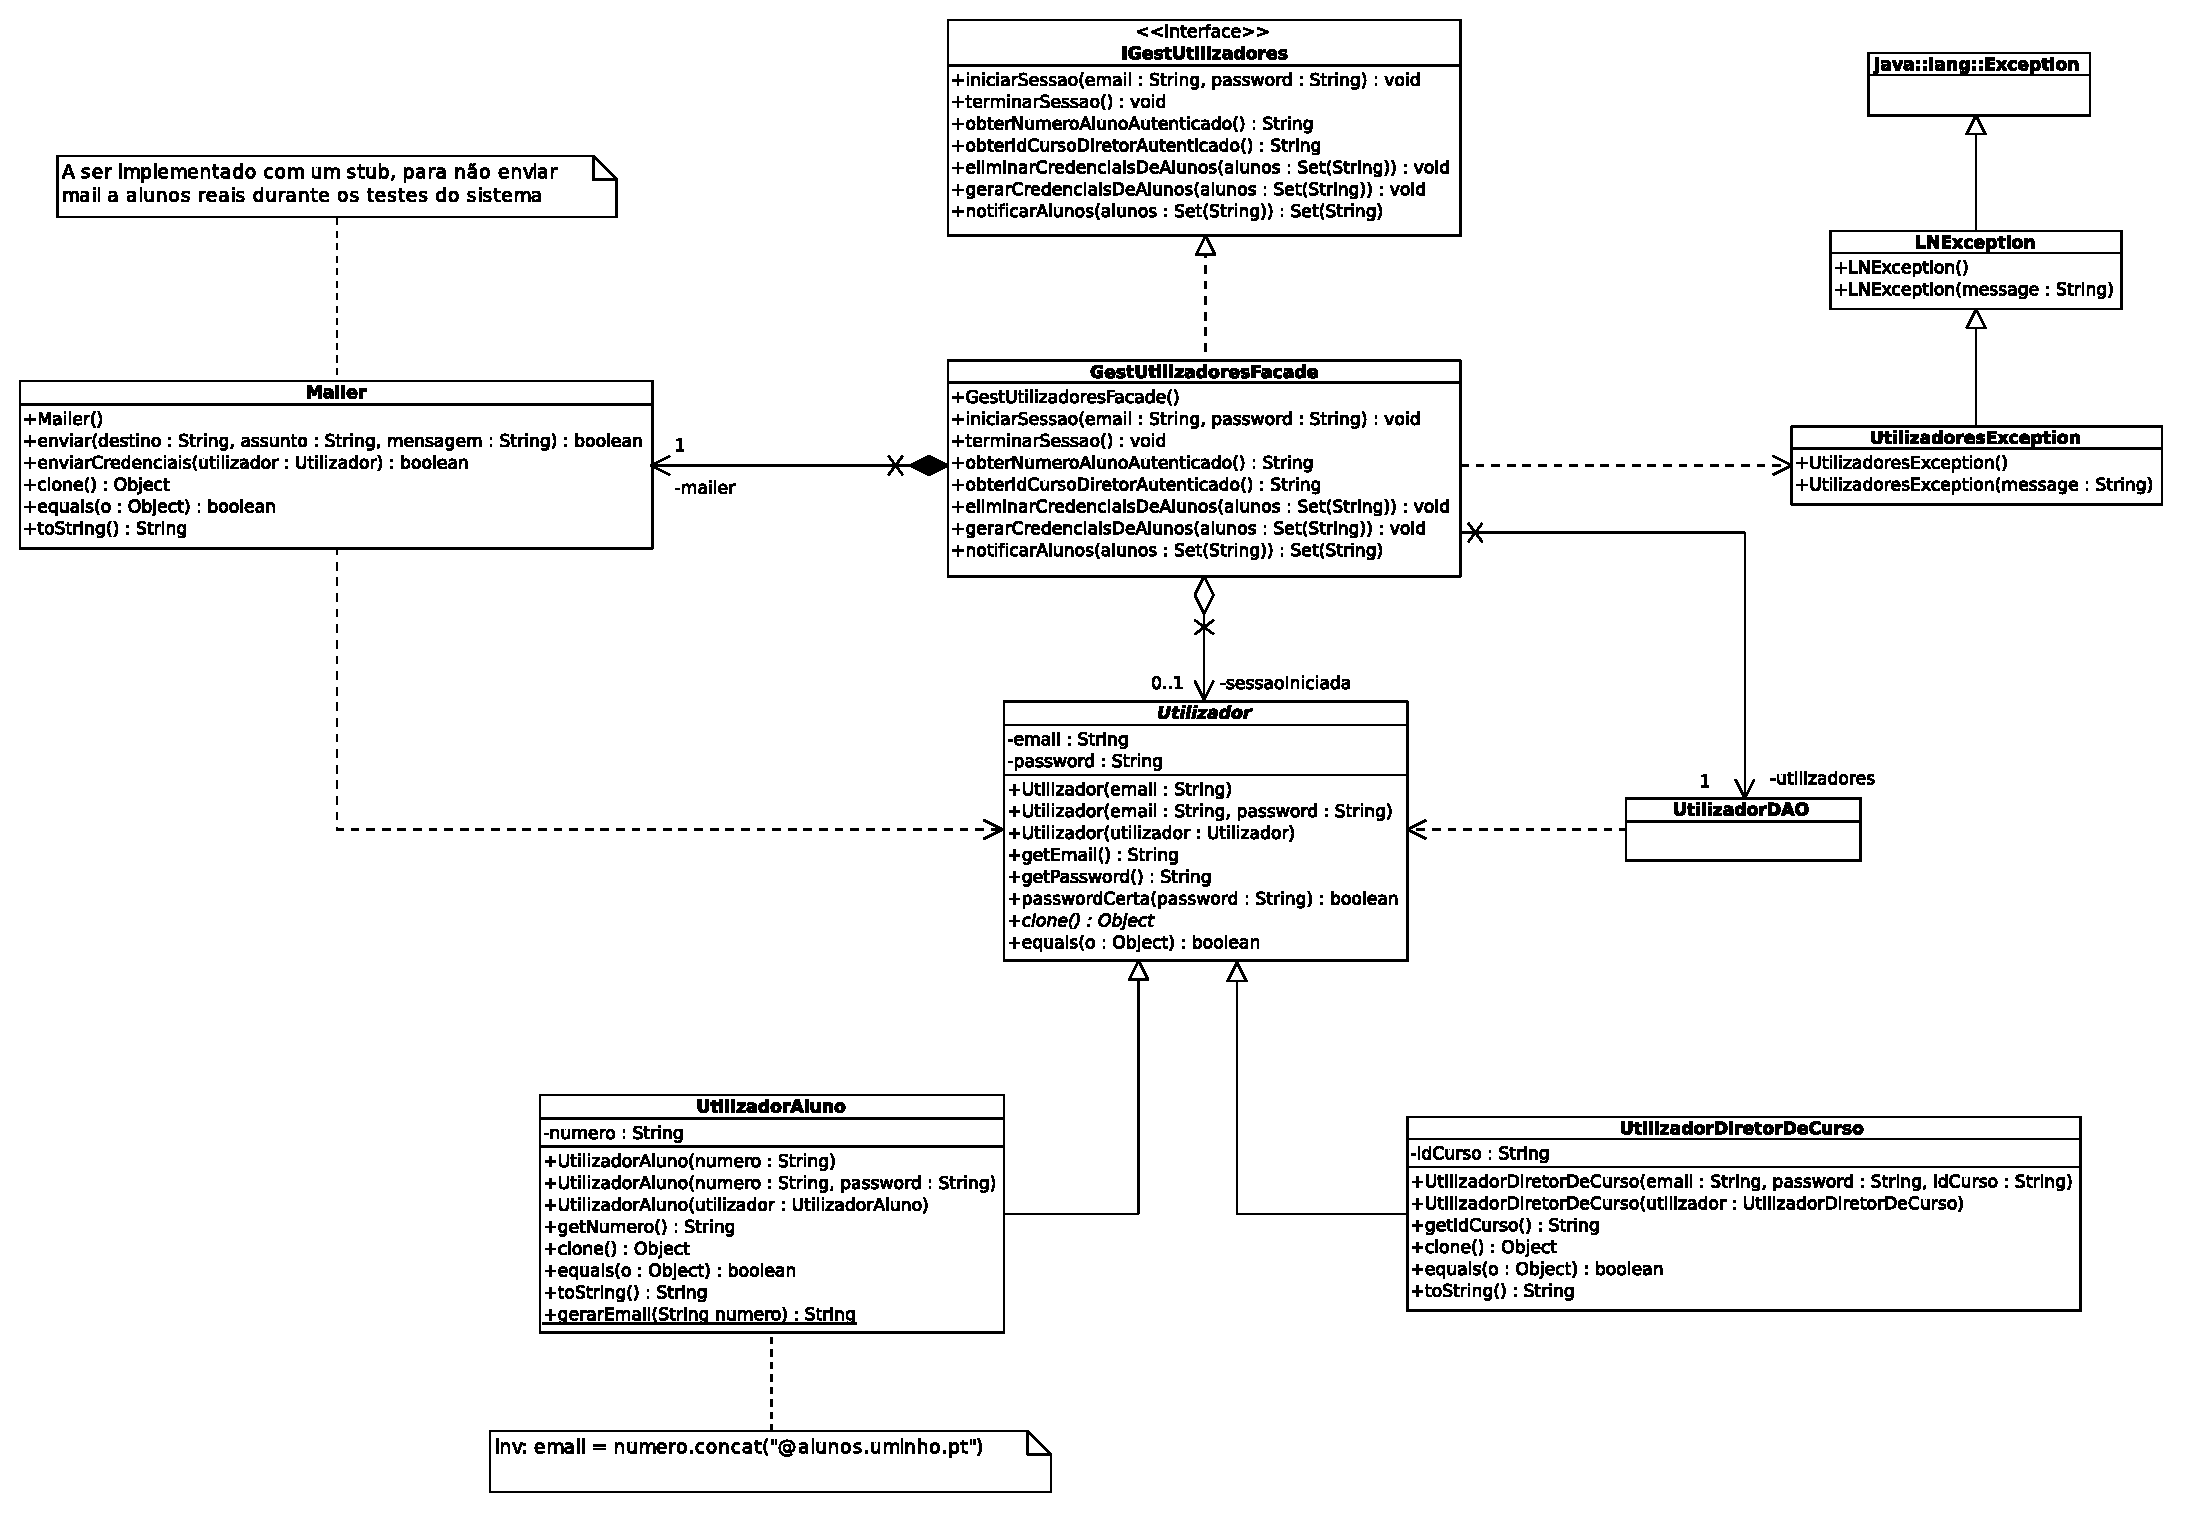
\includegraphics[width=0.7\textwidth]{Imagens/Modelos/UtilizadoresDAO.svg.eps} \\
    {\scriptsize Diagrama de classes do subsistema dos utilizadores após adição de DAOs}

    \vspace{0.5cm}
    \begin{itemize}
        \item Substituição de associações qualificadas pelo uso dos DAOs;
    \end{itemize}
\end{frame}

\begin{frame}{Implementação -- Alterações aos Diagramas de Sequência}
    \begin{itemize}
        \item Adição de atualizações à base de dados (\texttt{put}s nos DAOs);
        \item Alteração a alguns métodos internos das classes;
    \end{itemize}
\end{frame}

\begin{frame}{Implementação -- Camada de Apresentação}
    \centering

    \begin{itemize}
        \item Desenvolvimento da camada de apresentação na arquitetura MVC;
        \item Composição de um manual de instruções para os utilizadores.
    \end{itemize}
    \vspace{0.5cm}

    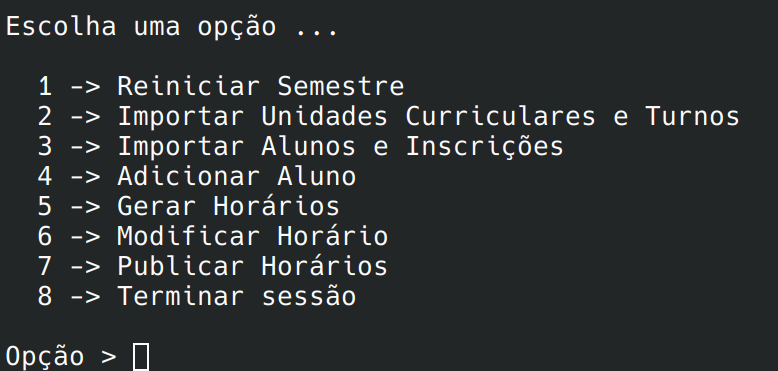
\includegraphics[width=0.7\textwidth]{Imagens/Manual/DiretorCurso.png} \\
    {\scriptsize Menu principal para diretores de curso.}
\end{frame}

\begin{frame}{Implementação -- Diagrama de Instalação}
    \centering
    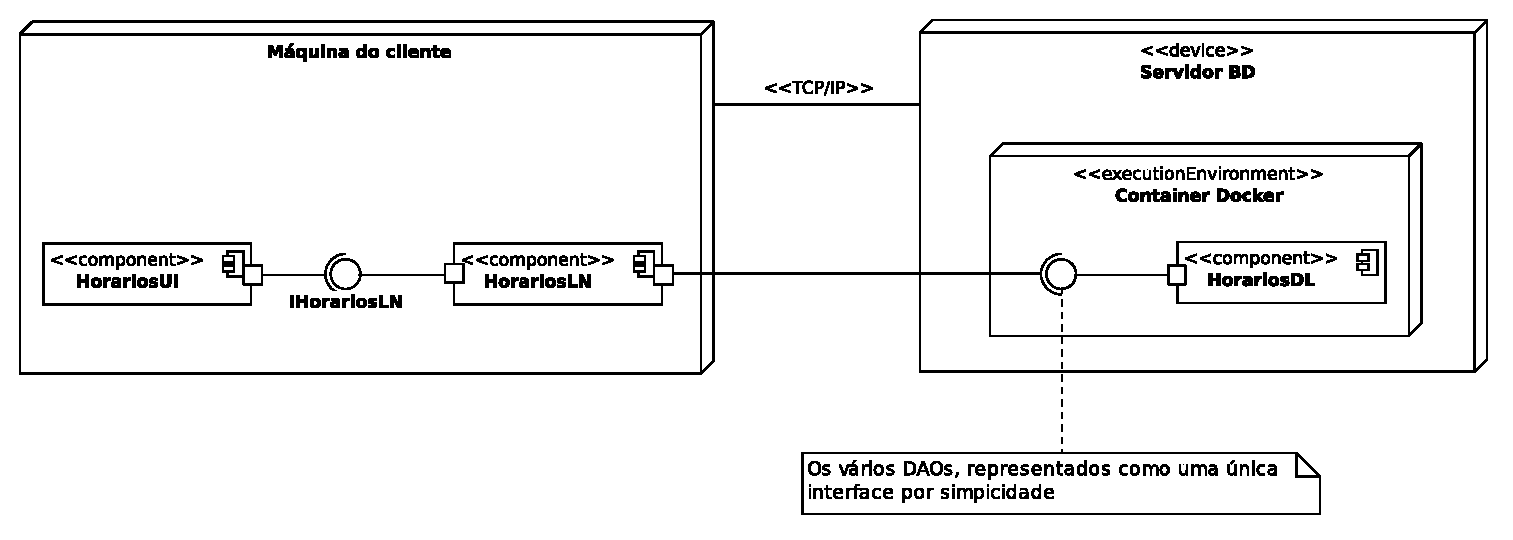
\includegraphics[width=\textwidth]{Imagens/Modelos/Instalação.svg.eps} \\
    {\scriptsize Diagrama de instalação construído.}

    \vspace{0.5cm}
    \begin{itemize}
        \justifying
        \item A ausência de tipos complexos permite uma fácil futura transferência da LN para outra
            máquina.
        \item A independência entre os subsistema permite uma fácil futura transição para uma
            arquitetura de micro-serviços.
    \end{itemize}
\end{frame}

\section{Apresentação do Produto Final}

\begin{frame}{Apresentação do Produto Final}
\end{frame}

\section{Conclusão}

\begin{frame}{Conclusão}
    Apesar de algumas dificuldades (divisão em subsistemas, implementação de preferências das UCs e
    adição de DAOs), sentimos que conseguimos desenvolver um sistema capaz de usar em ambientes
    reais e pelo próprio professor António Sousa.
\end{frame}

\frame{\titlepage}

\end{document}
